% Cover lengths
\newlength{\cH}\setlength{\cH}{.88\paperheight}% cover height
\newlength{\cW}\setlength{\cW}{0.600000000\cH}% cover width 3/5
\newlength{\cp}\setlength{\cp}{0.011965812\cH}% cover padding 7/585
\newlength{\ch}\setlength{\ch}{0.115213675\cH}% header heigth 337/2925
\newlength{\cw}\setlength{\cw}{0.117692308\cH}% side friezes width 153/1300
\newlength{\cf}\setlength{\cf}{1.111111111\cw}% friezes heigth 10/9
\newlength{\cth}
  \setlength{\cth}{6\cw}
  \addtolength{\cth}{-1.5\cp}
\newlength{\ctw}
  \setlength{\ctw}{\cW}
  \addtolength{\ctw}{-2\cw}
\addtolength{\ctw}{-4\cp}

\newcommand{\chcolumn}{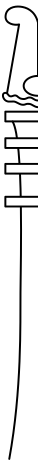
\includegraphics[width =0.5\cw]{cover/column-left-half}}
\newcommand{\chwings} {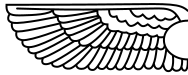
\includegraphics[width =2.5\ch]{cover/wings-left-half}}
\newcommand{\clfrieze}{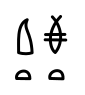
\includegraphics[height=   \cf]{cover/left-frieze}}
\newcommand{\crfrieze}{
\includegraphics[height=   \cf]{cover/right-frieze}}
\newcommand{\ccfrieze}{
\includegraphics[height=   \cf]{cover/center-frieze}}

\newcommand{\covertitling}{}

\newcommand{\ctitle}{
 \begin{minipage}[c][\cth][s]{\ctw}
  \centering\lineskip=0pt plus 1fill
  \vspace{\lineskip}
  \covertitling
  \vspace{\lineskip}
 \end{minipage}
}

\newcommand{\makecover}{
\clearpage
\thispagestyle{empty}
\begin{tikzpicture}[remember picture,overlay]
\node at (current page.center) {\begin{tikzpicture}
  % Decorations
  \node             at (     \cp +  0.5\cw,       \cp +.5\cf) {\clfrieze};
  \node             at (\cW -\cp -  0.5\cw,       \cp +.5\cf) {\crfrieze};
  \node             at (            0.5\cW,       \cp +.5\cf) {\ccfrieze};
  \node             at (     \cp +1.255\ch, \cH - \cp -.5\ch) {\chwings};
  \node [xscale=-1] at (     \cp +3.745\ch, \cH - \cp -.5\ch) {\chwings};
  \node             at (     \cp +0.252\cw, \cf +2\cp + 3\cw) {\chcolumn};
  \node [xscale=-1] at (     \cp +0.748\cw, \cf +2\cp + 3\cw) {\chcolumn};
  \node             at (\cW -\cp -0.748\cw, \cf +2\cp + 3\cw) {\chcolumn};
  \node [xscale=-1] at (\cW -\cp -0.252\cw, \cf +2\cp + 3\cw) {\chcolumn};
  % Frames
  \draw [black, solid, ultra thick] (0,0) rectangle ++(\cW,\cH);
  \draw [black, solid, ultra thick] (    \cp,\cp) rectangle ++( \cw,\cf);
  \draw [black, solid, ultra thick] (\cW-\cp,\cp) rectangle ++(-\cw,\cf);
  \draw [black, solid, ultra thick] (2\cp+\cw,\cp) rectangle ++(\cW-4\cp-2\cw,\cf);
  \draw [black, solid, ultra thick] (\cp,\cH-\cp) rectangle ++(5\ch,-\ch);
  \draw [black, solid, ultra thick] (\cw+2\cp,\cH-\ch-3.5\cp) rectangle (\cW-2\cp-\cw,\cH-6\cw-\ch-2\cp);
  \draw [black, solid, ultra thick] (\cp,\cH-2\cp-\ch) -- ++(0,-6\cw)
    -- ++(\cw,0) -- ++(0,6\cw-0.75\cp) -- ++(\cW-2\cw-2\cp,0)
    -- ++(0,-6\cw+0.75\cp) -- ++(\cw,0) -- ++(0,6\cw) -- cycle;
  % Titling
  \node at (0.5\cW,0.5\cH) {\ctitle};
\end{tikzpicture}};
\end{tikzpicture}
}
\clearpage

